\chapter{Modifiziertes RevPAR-Modell}
\label{sec:revpar}
In der vorherigen Sektion wurde ein vielversprechender Ansatz zur Identifizierung ähnlicher Hotels entwickelt und evaluiert, wobei erfolgreich der CatBoost-Algorithmus eingesetzt wurde, um präzise Vorhersagen über die Ähnlichkeit zwischen verschiedenen Hotels zu treffen. Basierend auf diesen Ergebnissen wird im folgenden Abschnitt ein neuer Schwerpunkt gesetzt, der darauf abzielt, die Erkenntnisse aus dem Ähnlichkeitsmodell zu nutzen und ein weiteres Modell zu entwickeln.
\newline
\newline 
Der Schwerpunkt dieser Sektion liegt auf der Modifikation des bereits vorhandenen RevPAR-Modells, das darauf abzielt, die RevPAR-Werte für ein Hotel vorherzusagen. Die vorgeschlagene Methode besteht darin, für jedes ähnliche Hotel ein eigenes RevPAR-Modell zu erstellen und den Durchschnitt der Ergebnisse zu ermitteln. Dabei werden die Daten der ähnlichen Hotels so angepasst, dass das Modell unabhängig vom spezifischen Hotel verwendet werden kann. Diese Sektion beginnt ebenfalls mit der Datenvorverarbeitung, bevor mit der Datenanalyse und Modellierung fortgefahren wird.

\subsection{Datenvorverarbeitung}
\label{subsec:revpar_prepare}
Die Datenvorverarbeitung dient dazu, zu ermitteln, welche Daten bereits vorhanden sind und wie sie modifiziert werden müssen, um die Entwicklung eines generellen Modells zu ermöglichen.

\begin{figure}[h]
    \centering
    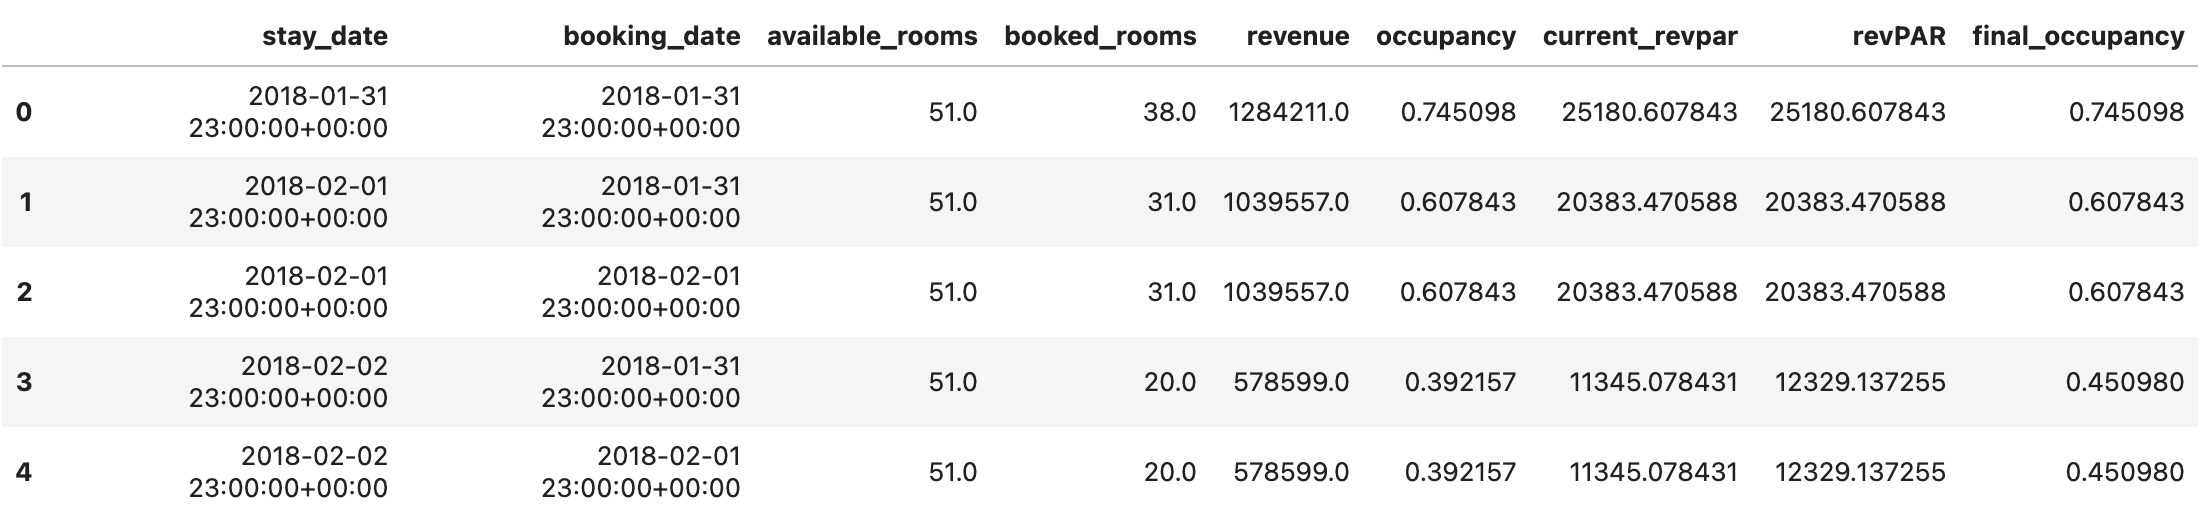
\includegraphics[width=1\textwidth, center]{revpar_features.png}
    \caption[Bereits vorhandene Hotelspezifischen Daten]{Bereits vorhandene Hotelspezifischen Daten}
    \label{img:revpar_features}
\end{figure}

Abbildung \ref{img:revpar_features} veranschaulicht beispielhaft die Vergangenheitsdaten, wie sie aus der Datenbank abgerufen werden können. Dabei repräsentiert die Spalte \emph{revPAR} den zu prognostizierenden Wert. Es ist zu erkennen, dass diese Werte sich spezifisch auf das ausgewählte Hotel beziehen und daher in ihrer aktuellen Form nicht für das Training verwendet werden können. Die vorgeschlagene Vorgehensweise besteht darin, sämtliche hotelspezifischen Spalten durch den Durchschnittswert der jeweiligen Spalte zu skalieren, um einen standardisierten Wert zu erlangen, der für jedes Hotel verwendet werden kann.
\newline 
\newline
Im Folgenden werden mehrere Funktionen definiert, die einerseits weitere Daten zum Datensatz hinzufügen sollen und andererseits die vorhandenen Spalten, wie oben beschrieben, durch den Durchschnittswert normieren sollen:

\begin{lstlisting}[language=Python, label=lst:revpar_helper_funcs, caption=Hilfsfunktions für das RevPAR Modell]
# list holiday
list_holidays = ['holiday_Neujahr', 'holiday_Christi Himmelfahrt','holiday_Erster Mai',
               'holiday_Karfreitag', 'holiday_Ostermontag','holiday_Pfingstmontag',
                 'holiday_Tag der Deutschen Einheit', 'holiday_Reformationstag', 'holiday_Erster Weihnachtstag', 
                 'holiday_Zweiter Weihnachtstag', 
                 ]

# list months
list_months = ['start_date_monthName_January', 'start_date_monthName_February', 'start_date_monthName_March', 
               'start_date_monthName_April', 'start_date_monthName_May', 'start_date_monthName_June',
               'start_date_monthName_July', 'start_date_monthName_August', 'start_date_monthName_September', 
               'start_date_monthName_October', 'start_date_monthName_November', 'start_date_monthName_December' ]

# list days
list_days = ['start_date_weekDayName_Monday', 'start_date_weekDayName_Tuesday', 'start_date_weekDayName_Wednesday',
            'start_date_weekDayName_Thursday', 'start_date_weekDayName_Friday', 'start_date_weekDayName_Saturday', 
             'start_date_weekDayName_Sunday']

# Vorbereiten der Hotelfeatures
def add_holidays_as_bool(df):
    ger_holidays = holidays.Germany()
    df['holiday'] = df.stay_date.apply(lambda x: ger_holidays.get(x.date()))
    df['holiday'] = df['holiday'].notnull().astype(int)
    return df

def add_month_feature(df):
    df.insert(loc=1, column='stay_date_monthName', value=df['stay_date'].dt.month_name())  
    return df

def add_weekDay_feature(df):
    df.insert(loc=1, column='stay_date_weekDayName', value=df['stay_date'].dt.day_name())
    return df

def add_year(df):
    df.insert(loc=1, column='stay_date_year', value=df['stay_date'].dt.year)
    return df

def feature_ADR(df):
    df['ADR'] = df['revenue'] / df['booked_rooms']
    df.loc[df['booked_rooms'] == 0, 'ADR'] = 0
    
    durchschnitt = np.mean(df['ADR'])
    df["scaled_current_adr"] = df['ADR'] / durchschnitt

    return df

def add_time_to_arrival(df):
    df['time_to_arrival'] = df['stay_date'] - df['booking_date']
    df['time_to_arrival'] = df['time_to_arrival'].dt.days
    return df

def add_stay_date_str(df):
    df["stay_date_str"] = df["stay_date"].dt.strftime("%d.%m.%Y")
    return df

def add_scaled_revpar_values(df):
    durchschnitt = np.mean(df['revPAR'])
    df["target"] = df['revPAR'] / durchschnitt
    df["scaled_current_revpar"] = df['current_revpar'] / durchschnitt
    return df
\end{lstlisting}

\begin{figure}[h]
    \centering
    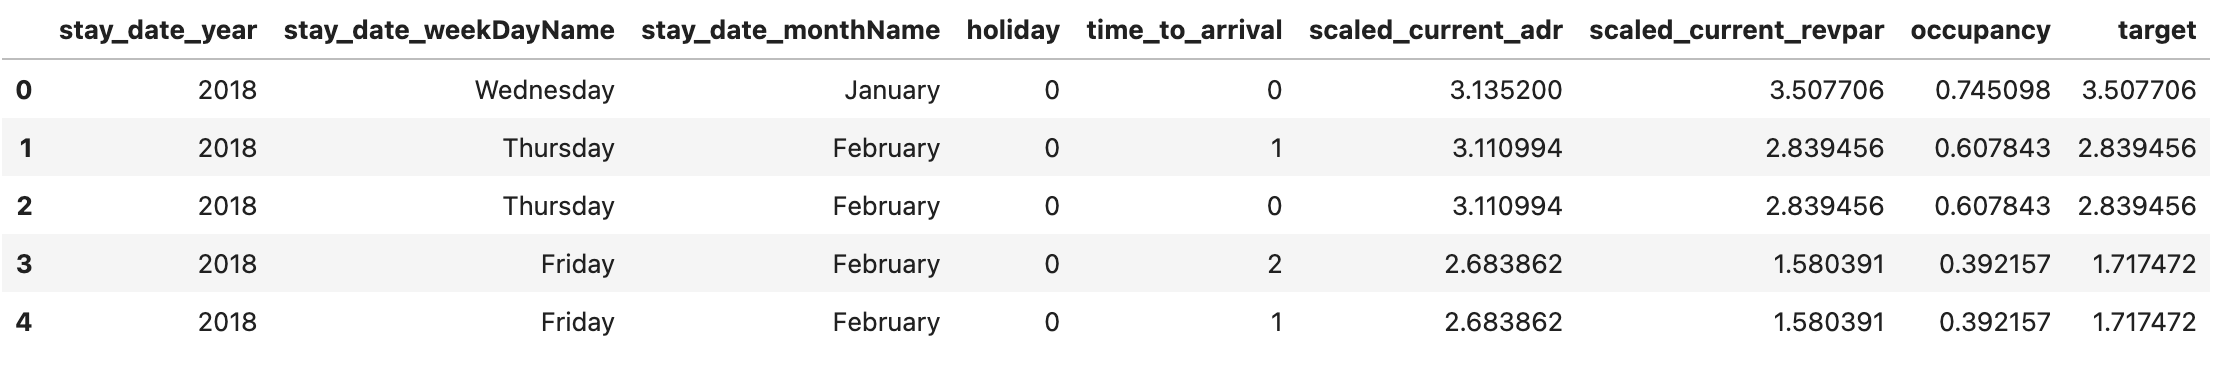
\includegraphics[width=1\textwidth, center]{revpar_features_2.png}
    \caption[Datensatz nach der Ausführung der Hilfsfunktionen]{Datensatz nach der Ausführung der Hilfsfunktionen}
    \label{img:revpar_features_2}
\end{figure}

Abbildung \ref{img:revpar_features_2} zeigt den Datensatz nach der Ausführung der Funktionen in Listing \ref{lst:revpar_helper_funcs}. Es ist zu erkennen, dass der Datensatz nun ausschließlich normierte Werte enthält. Im Folgenden wird eine Datenanalyse auf diesem Datensatz durchgeführt.

\subsection{Datenanalyse}
\label{subsec:revpar_analyse}

Wie bereits in Abschnitt \emph{\nameref{subsec:Datenanalyse}} erläutert wurde, ist die Datenanalyse eine der essenziellsten Komponenten bei der Modellierung eines Modells. Im Folgenden wird daher untersucht, welche hotelspezifischen Daten vorhanden sind und wie sie effektiv genutzt werden können.
\newline
\newline
Als erster Schritt soll erforscht werden, ob der gesamte Zeitraum des Datensatzes valide ist und verwendet werden kann. Dazu wird zunächst der durchschnittliche normierte RevPAR, repräsentiert durch die Spalte \emph{target}, mit den einzelnen Jahren verglichen.

\begin{figure}[h]
    \centering
    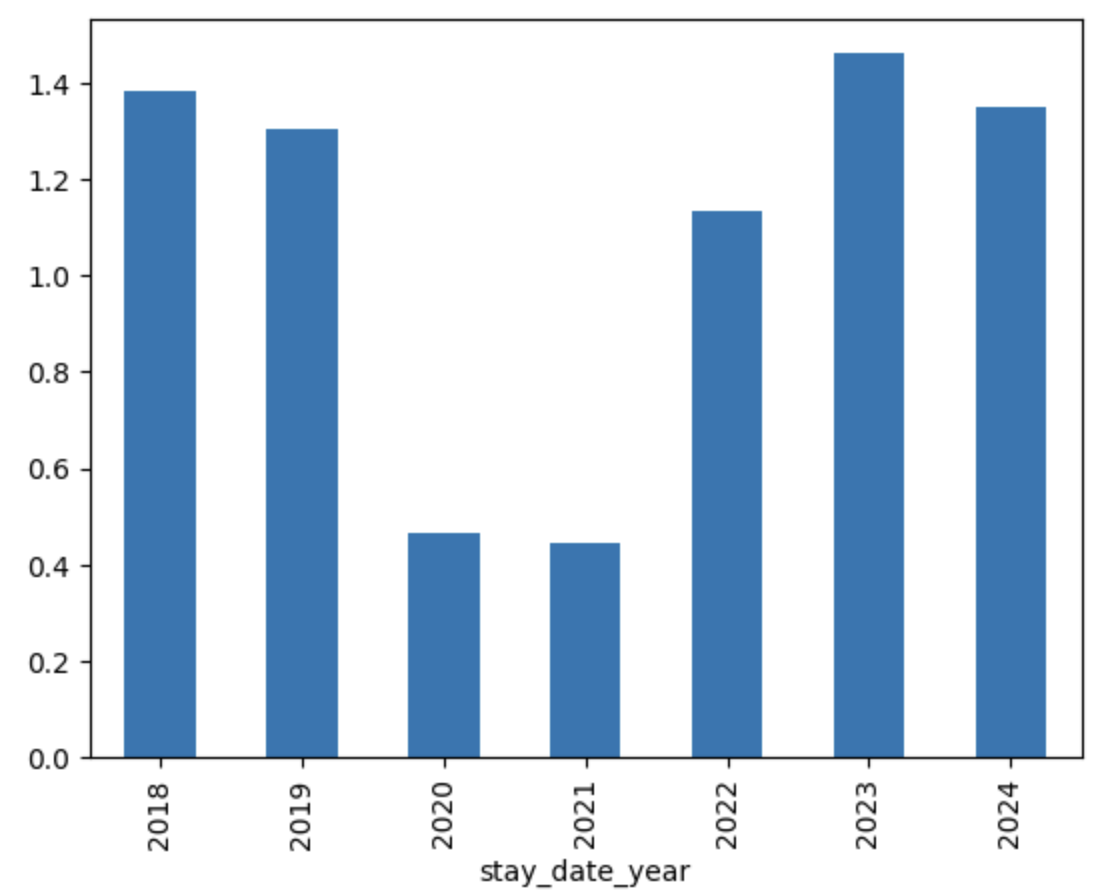
\includegraphics[width=1\textwidth, center]{revpar_target_year.png}
    \caption[Durchschnittlich normierte RevPAR-Werte pro Jahr]{Durchschnittlich normierte RevPAR-Werte pro Jahr}
    \label{img:revpar_target_year}
\end{figure}

Eine bedeutsame Erkenntnis aus Abbildung \ref{img:revpar_target_year} ist, dass nicht alle Jahre gleich sind. Insbesondere weisen die Jahre 2020 und 2021 einen deutlich niedrigeren durchschnittlichen RevPAR auf als die anderen Jahre. Diese Unterschiede können auf verschiedene Faktoren zurückzuführen sein, wobei die Zeit der Covid-19-Pandemie einen wesentlichen Beitrag zu dieser Abweichung geleistet haben dürfte, da viele Hotels zu dieser Zeit vorübergehend schließen mussten. Es wäre daher unangemessen, diese Informationen in das Modell einzubeziehen, da sie den Datensatz verfälschen würden. Da die Spalte 
\emph{stay\_date\_year}außer Ausreißern keine weiteren relevanten Informationen bietet, wird dieses Feature im weiteren Verlauf aus dem Datensatz entfernt.
\newline
\newline
Des Weiteren soll mit derselben Methodik überprüft werden, ob die Features
\newline 
\emph{stay\_date\_weekDayName}, \emph{stay\_date\_monthName} und \emph{holiday} einen signifikanten Einfluss auf den normierten RevPAR haben.

\newpage
\begin{figure}[h]
    \centering
    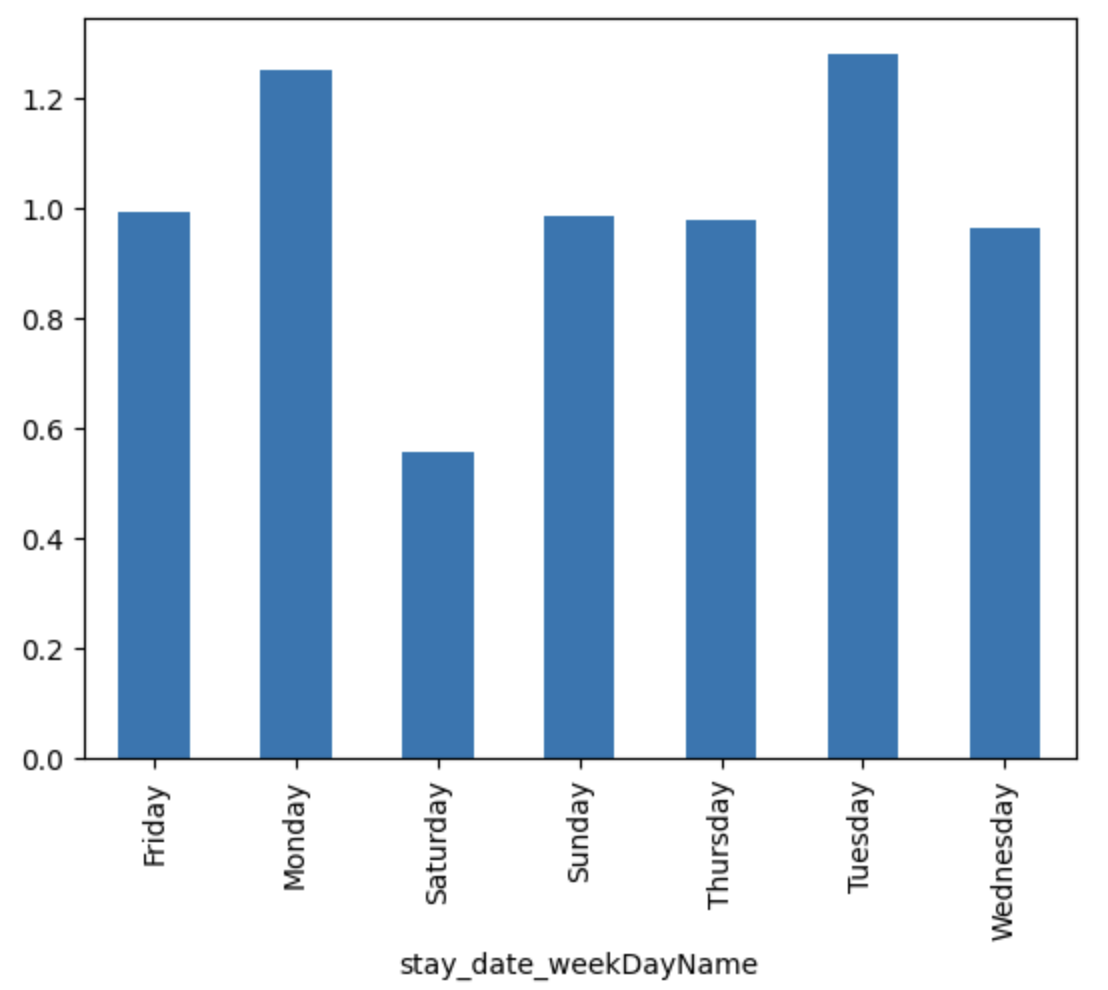
\includegraphics[width=0.6\textwidth, center]{revpar_target_week.png}
    \caption[Durchschnittlich normierte RevPAR-Werte pro Tag]{Durchschnittlich normierte RevPAR-Werte pro Tag}
    \label{img:revpar_target_week}
\end{figure}

\begin{figure}[h]
    \centering
    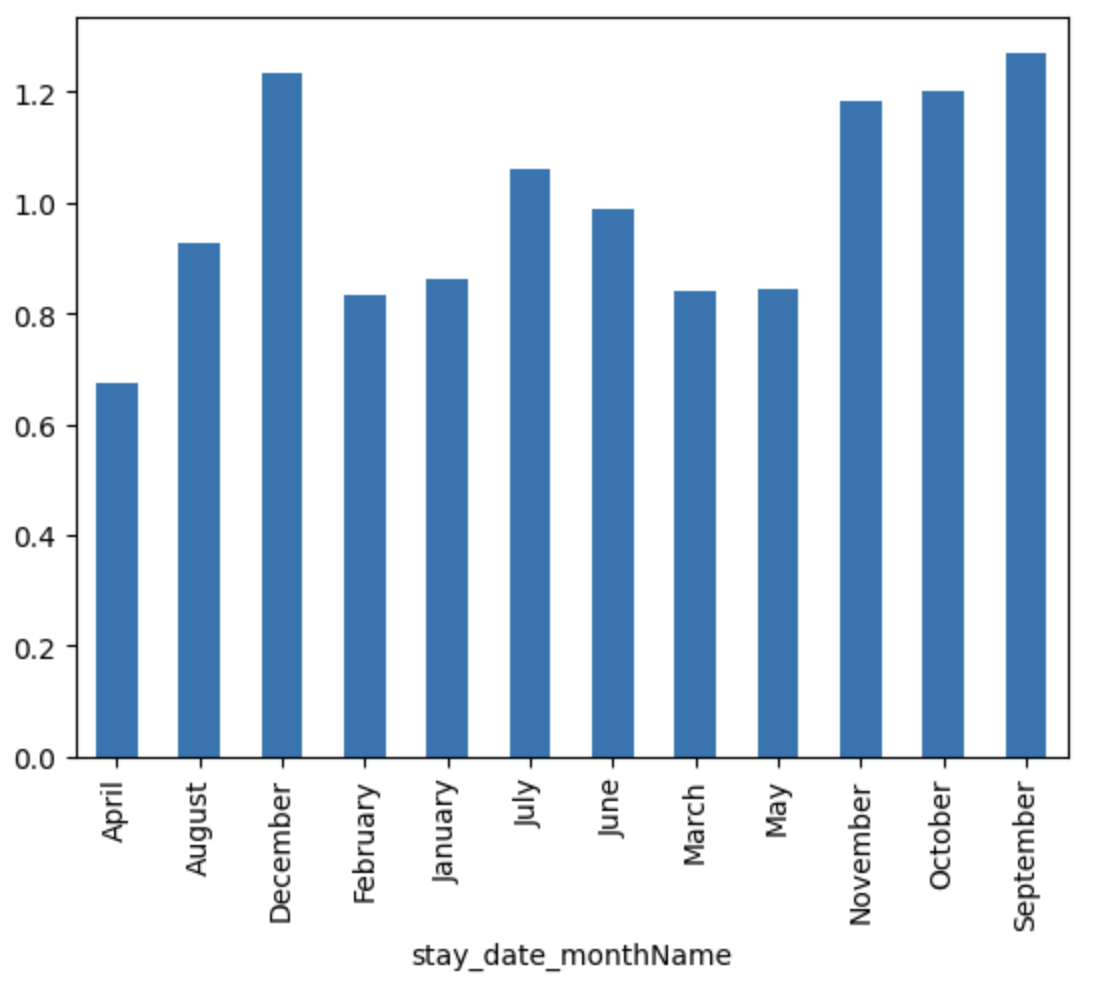
\includegraphics[width=0.6\textwidth, center]{revpar_target_month.png}
    \caption[Durchschnittlich normierte RevPAR-Werte pro Monat]{Durchschnittlich normierte RevPAR-Werte pro Monat}
    \label{img:revpar_target_month}
\end{figure}

\newpage

\begin{figure}[h]
    \centering
    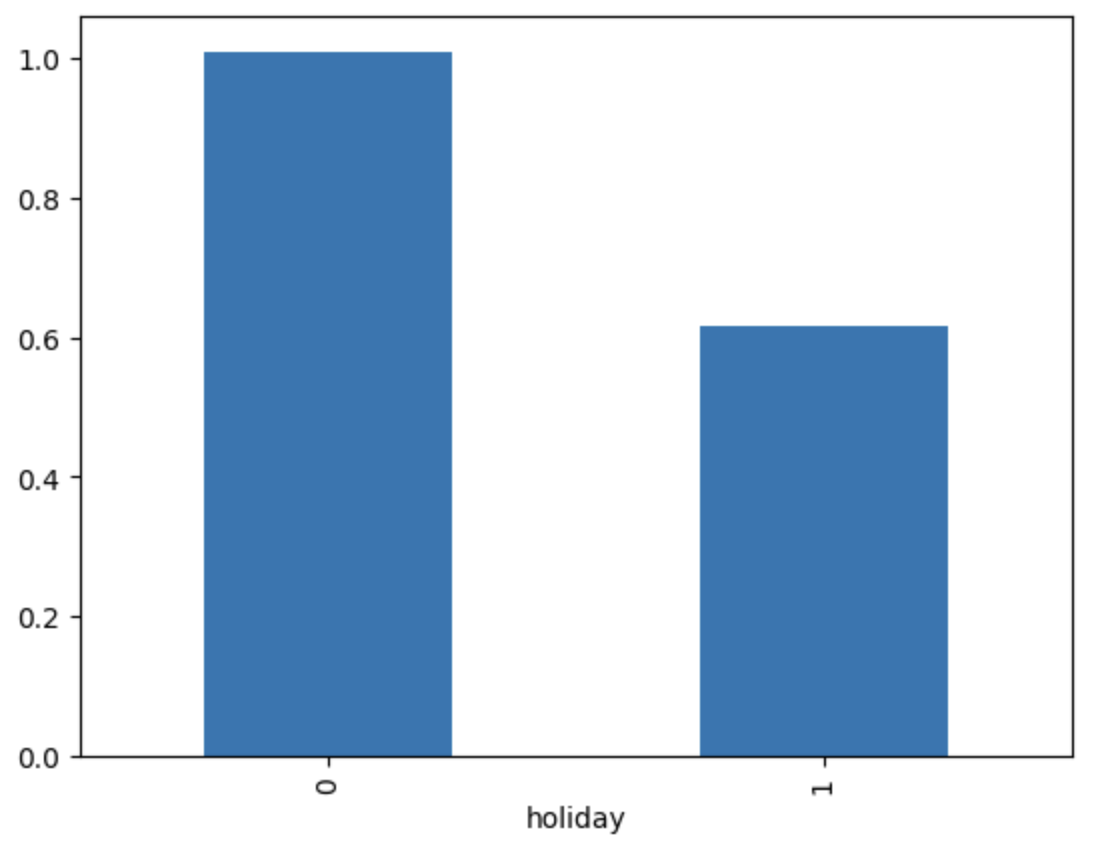
\includegraphics[width=0.6\textwidth, center]{revpar_target_holiday.png}
    \caption[Durchschnittlich normierte RevPAR-Werte Ferientage vs. nicht-Ferientage]{Durchschnittlich normierte RevPAR-Werte Ferientage vs. nicht-Ferientage}
    \label{img:revpar_target_holiday}
\end{figure}

Anhand der Abbildungen \ref{img:revpar_target_week}, \ref{img:revpar_target_month} und \ref{img:revpar_target_holiday} lässt sich erkennen, dass jedes dieser Features einen signifikanten Einfluss auf den normierten RevPAR hat und daher im Datensatz beibehalten werden sollte.
\newline 
\newline
Zum Abschluss sollen noch die Spalten \emph{scaled\_current\_adr}, \emph{scaled\_current\_revpar} und \emph{occupancy} auf ihren Einfluss überprüft werden. Hierzu wird im Folgenden eine Korrelationsmatrix erstellt, um die Korrelation dieser Spalten mit dem normierten RevPAR zu bestimmen.

\begin{figure}[h]
    \centering
    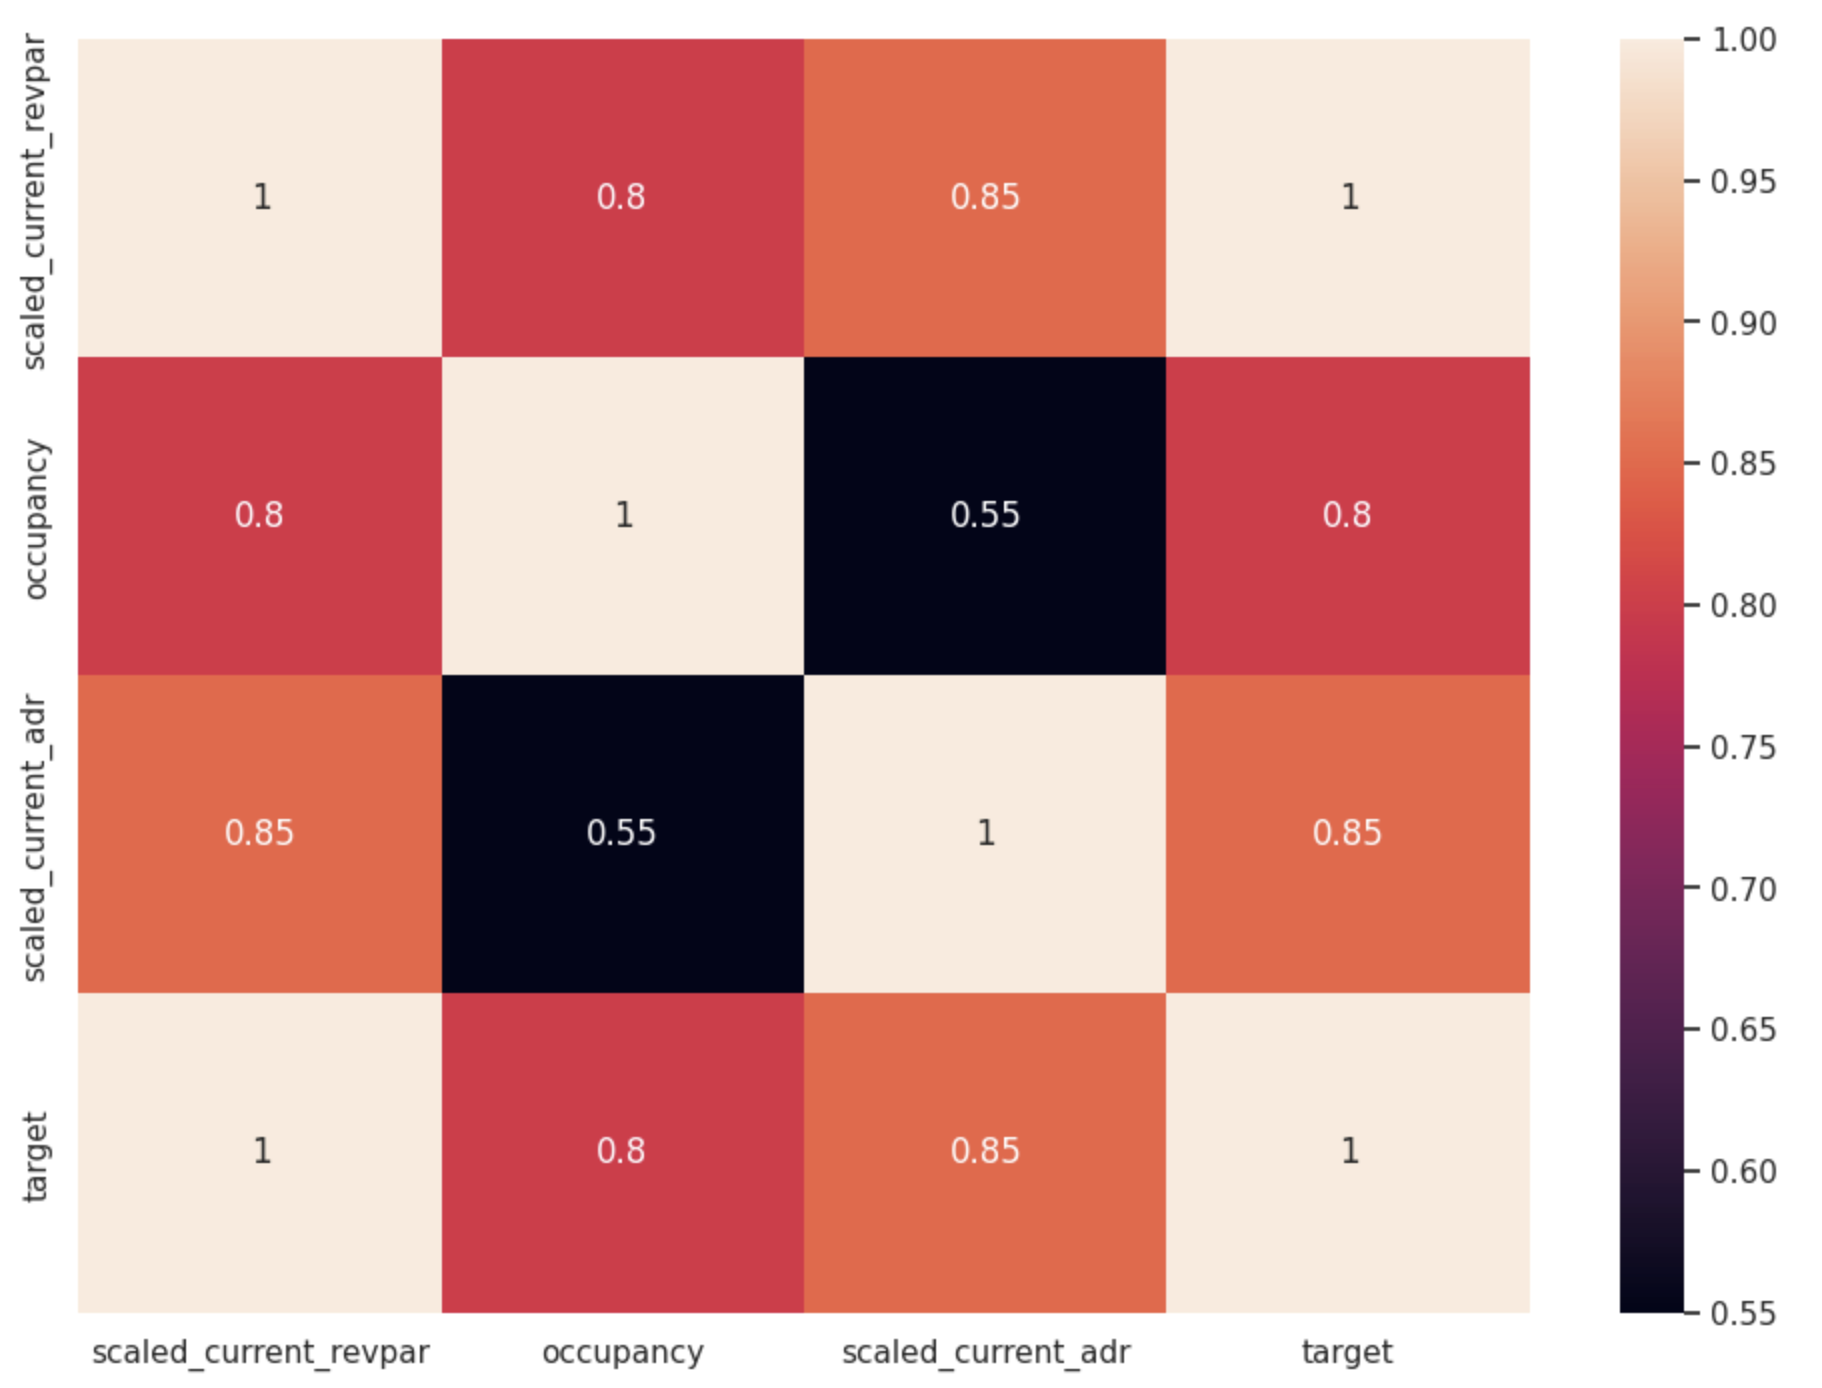
\includegraphics[width=0.6\textwidth, center]{revpar_corr.png}
    \caption[Korrelationsmatrix der verbleibenden Spalten]{Korrelationsmatrix der verbleibenden Spalten}
    \label{img:revpar_corr}
\end{figure}

Bei Betrachtung der unteren Zeile \emph{target} ist festzustellen, dass alle aufgelisteten Features eine signifikante Korrelation zur Zielvariable aufweisen. Daher sollten sie auch im Datensatz berücksichtigt werden.
\newline 
\newline 
Der resultierende Datensatz, welche nach der Entfernung der Ausreißer und unnötigen Feature entsteht sieht wie folgt aus:

\begin{figure}[h]
    \centering
    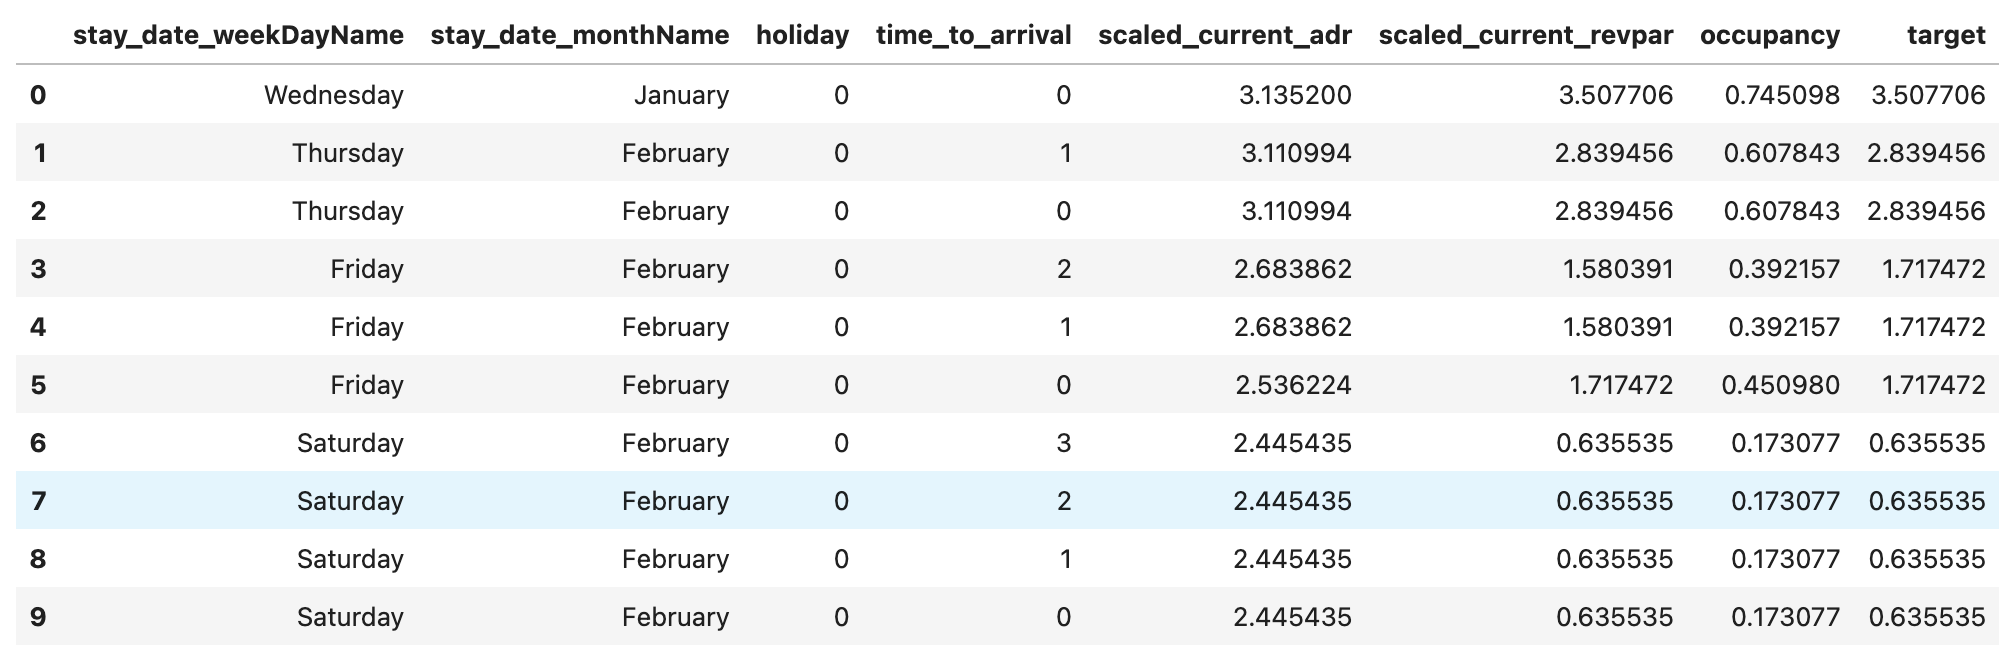
\includegraphics[width=1\textwidth, center]{revpar_df.png}
    \caption[Finaler Datensatz für das RevPAR-Modell]{Finaler Datensatz für das RevPAR-Modell}
    \label{img:revpar_df}
\end{figure}

\section{Modellbildung}
\label{subsec:revpar_model}

Nachdem der vorbereitete Datensatz vorliegt, wird das Modell implementiert. Aufgrund des Vorhandenseins vieler kategorischer Daten wird erneut das CatBoost-Modell verwendet. Die Implementierung erfolgt ähnlich wie in der vorherigen Sektion zur Identifizierung ähnlicher Hotels.

\begin{lstlisting}[language=Python, label=lst:revpar_model, caption=Erzeugung der RevPAR-Vorhersagen]
import catboost as cb

cat_features = [
    "stay_date_weekDayName",
    "stay_date_monthName",
    "holiday",
    "time_to_arrival"
]
    
result_dict = dict()
    
for id in silimar_hotel_ids:
    X_train, y_train, X_test, y_test = get_data(id)
    model = cb.CatBoostRegressor()
    model.fit(X_train, y_train, cat_features=cat_features)
    y_pred = model.predict(X_test)
    result_dict[id] = y_pred
    
df = pd.DataFrame(result_dict)
overall_preds = df.astype(float).mean(axis=1)
\end{lstlisting}

Die Code-Zeilen in Listing \ref{lst:revpar_model} erzeugen die Variable \emph{overall\_preds}, die eine Liste von normierten RevPAR-Werten darstellt. Diese normierten RevPAR-Werte werden als Vorhersage für das Hotel ohne Vergangenheitsdaten verwendet.
    
\subsection{Evaluation}
\label{subsec:revpar_eval}
Nachdem im vorherigen Abschnitt die Vorhersage normierter RevPAR-Werte mittels eines definierten Code-Abschnitts erfolgte, rückt nun die Frage nach der Genauigkeit dieser Vorhersagen in den Vordergrund. Diese Sektion widmet sich daher einer eingehenden Untersuchung der Wirksamkeit der vorhergesagten Werte für das Jahr 2023. Ziel dieser Evaluation ist es, die Übereinstimmung der prognostizierten Werte mit den tatsächlichen Daten zu bewerten und die Zuverlässigkeit des Modells bei der Vorhersage zu prüfen.
\newline
\newline
Um dieses Ziel zu erreichen, werden verschiedene Metriken wie der R2-Score, der Root-Mean-Square-Error und der Mean-Absolute-Error verwendet, um die Abweichungen zwischen den Vorhersagen und den realen Werten zu quantifizieren. Darüber hinaus erfolgt ein direkter Vergleich zwischen dem entwickelten Modell und dem aktuellen Live-Modell, das derzeit von Kunden verwendet wird. Diese Gegenüberstellung ermöglicht es, fundierte Entscheidungen über das weitere Vorgehen zu treffen, basierend auf einem direkten Vergleich der Leistungsfähigkeit beider Modelle.

\begin{figure}[h]
    \centering
    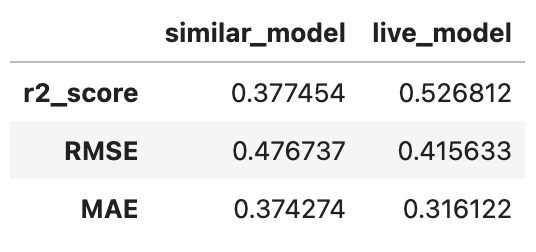
\includegraphics[width=0.5\textwidth, center]{revpar_eval_1.png}
    \caption[Evaluation der beiden Modelle für das erste Benchmark-Hotel]{Evaluation der beiden Modelle für das erste Benchmark-Hotel}
    \label{img:revpar_eval_1}
\end{figure}

Die Darstellung in Abbildung \ref{img:revpar_eval_1} präsentiert die Ergebnisse der einzelnen Modelle und ermöglicht gleichzeitig einen direkten Vergleich zwischen ihnen. Dabei fällt auf, dass das aktuell verwendete Live-Modell im Vergleich zum Similar-Modell eine bessere Leistung für dieses spezifische Hotel aufweist. Es ist jedoch wichtig zu beachten, dass das Similar-Modell gänzlich auf hotel-spezifische Daten verzichtet und trotzdem nur eine geringfügige Differenz aufweist.
\newline
\newline
Die Berücksichtigung eines einzelnen Hotels allein für diese Evaluation könnte als begrenzt angesehen werden. Daher wird die Analyse um das zweite Benchmark-Hotel erweitert, um festzustellen, wie die einzelnen Modelle dort abschneiden. Dies ermöglicht eine umfassendere Beurteilung der Leistungsfähigkeit der Modelle über verschiedene Kontexte hinweg.

\begin{figure}[h]
    \centering
    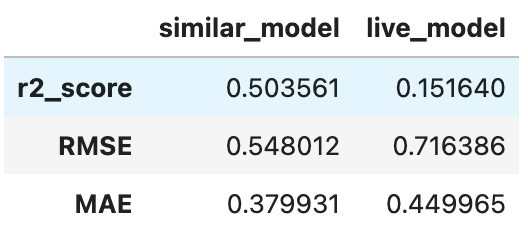
\includegraphics[width=0.5\textwidth, center]{revpar_eval_2.png}
    \caption[Evaluation der beiden Modelle für das zweiten Benchmark-Hotel]{Evaluation der beiden Modelle für das zweiten Benchmark-Hotel}
    \label{img:revpar_eval_2}
\end{figure}

Die Einbeziehung der Ergebnisse des zweiten Benchmark-Hotels, wie sie in Abbildung \ref{img:revpar_eval_2} dargestellt sind, verdeutlicht signifikante Unterschiede in der Leistung des Live-Modells. In diesem Szenario erweist sich das Similar-Modell als deutlich überlegen, obwohl es ohne hotel-spezifische Daten arbeitet. Diese Erkenntnis unterstreicht, dass die Modelle je nach individuellen Hotelkontexten unterschiedlich gut abschneiden können.

\subsection{Zwischenfazit}
\label{subsec:revpar_fazit}
Die präsentierten Ergebnisse in Abschnitt \emph{\nameref{subsec:revpar_eval}} legen nahe, dass das Similar-Modell trotz des Fehlens hotel-spezifischer Daten einen validen Ansatz zur Vorhersage normierter RevPAR-Werte darstellt. Basierend auf diesen Erkenntnissen wurde beschlossen, diesen Ansatz für die dynamische Preisgenerierung von Hotels ohne Verfügbarkeit von Vergangenheitsdaten zu nutzen.


\section{Dynamische Preisgenerierung}
\label{subsec:revpar_price}
Durch die Implementierung des Modells in der vorherigen Sektion werden normierte RevPAR-Werte generiert, die in einem DataFrame wie folgt dargestellt werden können:

\begin{figure}[h]
    \centering
    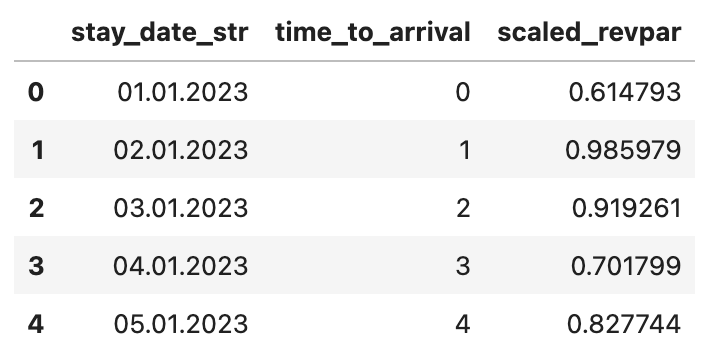
\includegraphics[width=1\textwidth, center]{revpar_price_1.png}
    \caption[Datensatz der Vorhersage]{Datensatz der Vorhersage}
    \label{img:revpar_price_1}
\end{figure}

Um die tatsächlichen Preise unter Verwendung des RevPAR-Preis-Mappings für die einzelnen Zimmerkategorien zu generieren, ist es erforderlich, die normierten RevPAR-Werte in ihre ursprüngliche Form zu überführen. Dies erfolgt durch die Multiplikation der normierten RevPAR-Werte mit dem durchschnittlichen RevPAR-Wert des Hotels. Zu diesem Zweck wird dem DataFrame eine zusätzliche Spalte mit dem Namen \emph{revpar} hinzugefügt. Diese Spalte repräsentiert das Produkt aus dem normierten RevPAR und dem durchschnittlichen RevPAR des Hotels.

\begin{figure}[h]
    \centering
    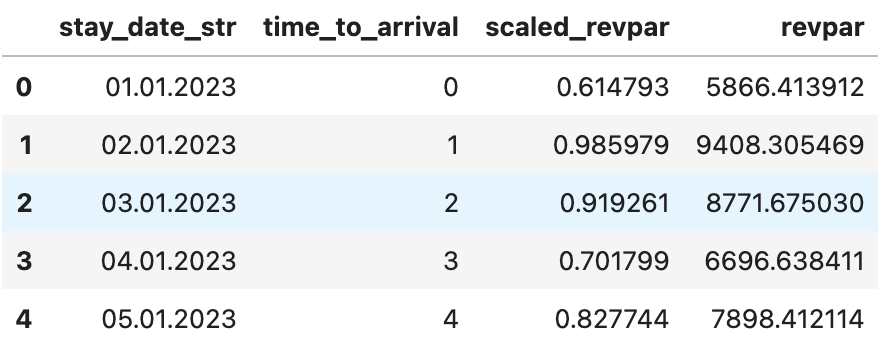
\includegraphics[width=1\textwidth, center]{revpar_price_2.png}
    \caption[Datensatz mit dem tatsächlichen RevPAR-Werten]{Datensatz mit dem tatsächlichen RevPAR-Werten}
    \label{img:revpar_price_2}
\end{figure}

Durch diese Vorgehensweise wurde eine vergleichbare Ausgangssituation wie beim ursprünglichen RevPAR-Modell geschaffen. Von diesem Punkt an kann das Mapping vom RevPAR-Wert zum Preis verwendet werden, um die tatsächlichen Zimmerpreise zu generieren.
\newpage
\begin{figure}[h]
    \centering
    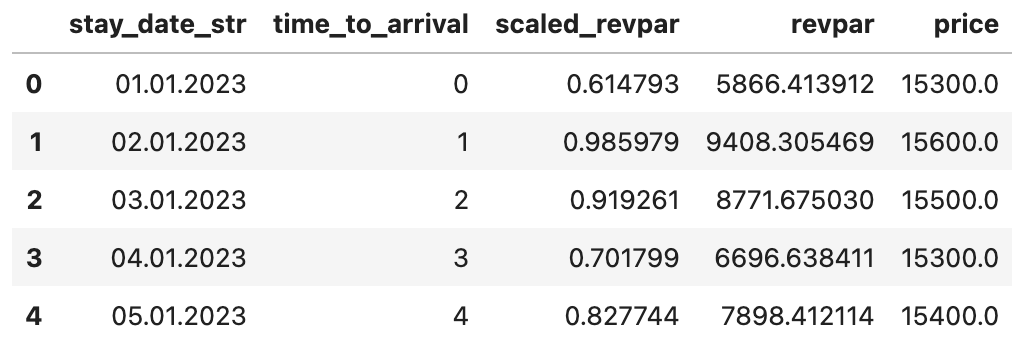
\includegraphics[width=1\textwidth, center]{revpar_price_3.png}
    \caption[Datensatz mit dem tatsächlichen Preisen]{Datensatz mit dem tatsächlichen Preisen}
    \label{img:revpar_price_3}
\end{figure}

Die Abbildung \ref{img:revpar_price_3} zeigt beispielhaft die Preise in Cent für eine bestimmte Zimmerkategorie, die schließlich dem Kunden vorgeschlagen werden.